\documentclass[]{article}
\usepackage[utf8]{inputenc}
\usepackage{graphicx}
\usepackage{lipsum}
%\usepackage[utf8]{inputenc}
%\usepackage{graphicx}
\usepackage{amsmath}
\usepackage{amssymb}
\usepackage{physics}
\usepackage{tcolorbox}
\usepackage{color}   %May be necessary if you want to color links
\usepackage[hidelinks]{hyperref}
\usepackage{mathtools}
\usepackage{graphicx} % Allows including images
\usepackage{booktabs} % Allows the use of \toprule, \midrule and \bottomrule in tables
\usepackage{calligra}

\DeclareMathAlphabet{\mathcalligra}{T1}{calligra}{m}{n}
\DeclareFontShape{T1}{calligra}{m}{n}{<->s*[2.2]callig15}{}
\newcommand{\scriptr}{\mathcalligra{r}\,}
\newcommand{\boldscriptr}{\pmb{\mathcalligra{r}}\,}

\graphicspath{ {images/} }

%opening
\title{Vector Analysis}
\author{}

\begin{document}

\maketitle

%\begin{abstract}

%\end{abstract}
\section{Vector Algebra}


\section{Differential Calculus}
\subsection{"Ordinary" Derivatives}
What is the derivative of a function $f(x)$? It tells us how quickly f(x) changes when we make a small change $dx$ in it's argument $x$,
\begin{equation}
df = \left(\frac{df}{dx}\right) dx
\end{equation}
If we change $x$ by an amount $dx$ then $f(x)$ changes by an amount $df$, the derivative is a proportionality factor. Geometrically speaking, the derivative $df/dx$ is the slope/gradient of the graph of $f(x)$ versus $x$. 
\subsection{Gradient}
The gradient, geometrically speaking points in the diretion of maximum increase/ascent for the function 
\subsection{The Del Operator}
\subsection{The Divergence}
\subsection{The Curl}
\subsection{Product Rules}
\subsection{Second Derivatives}
\section{Integral Calculus}

\section{Curvilinear Coordinates}
\subsection{Spherical Coordinates}
\subsection{Cynlindrical Coordinates}
The cylindrical coordinates are related to the cartesian coordinates by the relations
\begin{equation}
	\begin{cases}
		x = &
		
	\end{cases}
\end{equation}
the unit vectors are,
The infinitesimal displacements are,
Line element,
Volume element,
Gradient,
Divergence

Curl,

\section{The Dirac Delta Function}
\subsection{The Divergence of $\frac{\hat{r}}{r^{2}}$}
We can see why the divergence is,
\begin{equation}
	\nabla . \frac{\hat{r}}{r^{2}} = 0
\end{equation}
But if we calculate this using the Divergence theorem, we find that 
\subsection{The One-Dimensional Dirac Delta Function}
The Dirac Delta is a functional \footnote{An object that is a map between functions} which we define as,
\begin{equation}
	\delta(x-a)= 
	\begin{cases}
		0, & \text{if } x \neq a\\
		\infty,              & \text{if } x = a
	\end{cases}
	\label{del1}
\end{equation}
\begin{equation}
	\int_{- \infty}^{+ \infty} \delta(x-a) dx = 1
	\label{del2}
\end{equation}
$\forall \  a \in \mathbb{R}$
We can visualize it as a sharp peak at $a$,
\begin{figure}
	\centering
	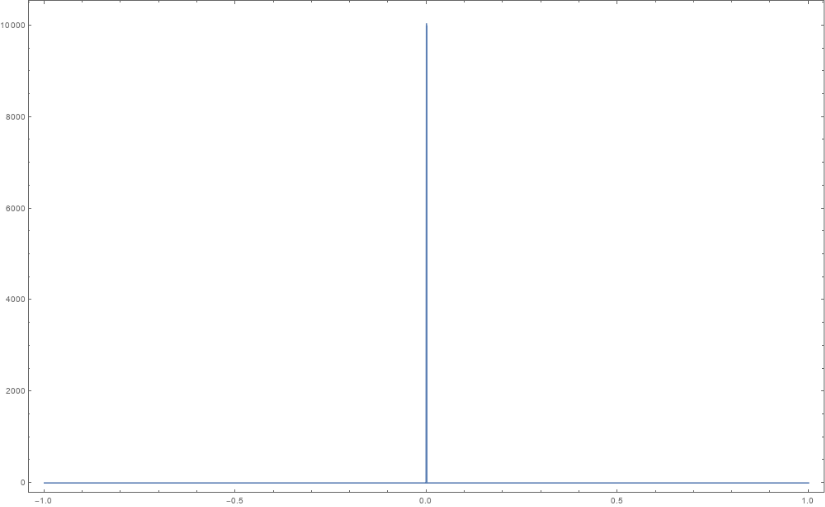
\includegraphics[scale=0.5]{delta-distribution.png}
	\caption{A Plot of $\delta(x)$}
\end{figure}
We can interpret \ref{del2} as saying "the area of the delta distribution is always 1".
\begin{equation}
	f(x)\delta(x - a ) = f(a)
\end{equation}
We can combine these to get,
\begin{equation}
	\int_{- \infty}^{+ \infty} \delta(x-a) f(x) dx = f(a)
\end{equation}
\subsubsection{A few interesting properties}
\begin{equation}
	\delta(kx) = \frac{1}{|k|}\delta(x)
\end{equation}
\begin{equation}
	\frac{d}{dx}(\delta(x)) = -\delta(x)
\end{equation}
where k is a constant
\begin{equation}
	\frac{d \theta}{dx} = \delta(x)
\end{equation}
Where $\theta$ is the step function defined as,
\begin{equation}
	\theta(x)= 
	\begin{cases}
		1, & \text{if } x > 0\\
		o,              & \text{if } x \leq 0
	\end{cases}
\end{equation}

\subsection{The Three-Dimensional Dirac Delta Function}
We generalize () to three dimensions,
\begin{equation}
	\delta^{3}(\vec{r} - \vec{a}) = \delta(x-a_{x})\delta(y-a_{y})\delta(z-a_{z})
\end{equation}
\begin{equation}
	\int_{- \infty}^{+ \infty} \delta^{3}(\vec{r} - \vec{a}) dV = 1
\end{equation}
We can also define the three-dimensional delta function as
\begin{equation}
	\delta^{3}(\boldscriptr) = \frac{1}{4 \pi} \left[\nabla \cdot \left( \frac{\hat{\boldscriptr}}{{\scriptr	}^{2}}\right)\right]
\end{equation}
Since,
$$\nabla \left(\frac{1}{\scriptr}\right) = -\frac{\hat{\boldscriptr}}{\scriptr^{2}}$$
We can rewrite as,
\begin{equation}
	\delta^{3}(\boldscriptr) = -\frac{1}{4 \pi} \left[\nabla^{2}  \left( \frac{1}{\scriptr}\right)\right]
\end{equation}
\section*{References}
\end{document}
